\chapter{Implementation}


%5\section{Extension Structure}

As explained in \ref{browserExtensions}, the extension is split into different files for both security reasons and other separation of concerns.
The diagram below puts into more detail the exact structure of the extension in context with some of the real files being used.


\begin{figure}[h]
	\centering
	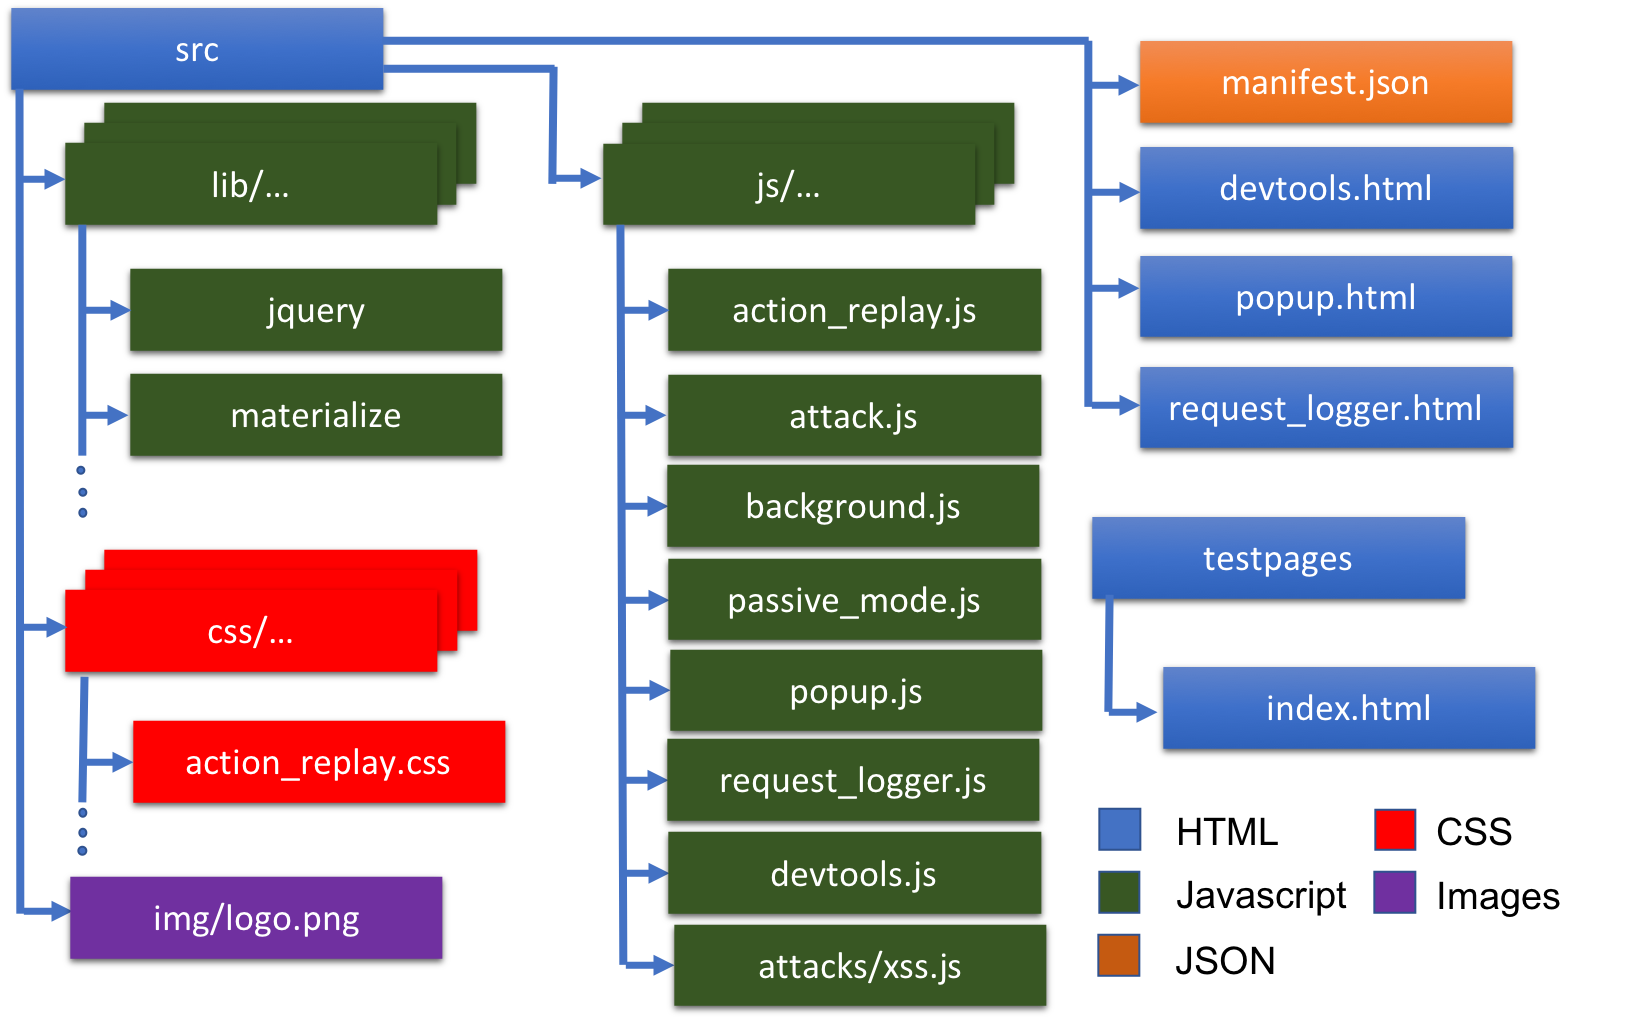
\includegraphics[width=0.9\textwidth]{images/project_structure.png}
	\caption{The directory structure used for the project}
	\label{fig:test}
\end{figure}

I have arranged the files in question into 2 separate subfolders - the \texttt{testpages} directory keeps the source code for the test harness page with vulnerabilities, while the \texttt{src} directory keeps all the other extension related code. \\

Within \texttt{src} we find different folders for separate concerns - \texttt{lib} stores any library code I have imported from a third-party, \texttt{css} keeps custom styles used across the extension, \texttt{img} is where any images are kept, \texttt{js} holds any custom produced Javascript files, and is where most of the logic within the extension lives. \texttt{src} also contains the \textit{manifest} file, and any HTML page code. 

\section{Manifest}

The manifest is where the extension declares its intentions by enumerating all the scripts and files to be accessed, as well as the permissions required to run the extension as an add-on to the browser. This file is necessary due to security reasons; each extension is expected to run as a standalone program within the browser. Any dependencies are to be declared and included within the package before the program is run, with the exception of contents that are whitelisted in the declared \textit{Content Security Policy} (CSP) directive within the file. I am using the recommended default CSP directive of \texttt{script-src 'self'; object-src 'self'}. This policy actively prevents notoriously dangerous Javascript functions from being evaluated, disables in-line Javascript functionality (which enforces a separation of content from behaviour), and, as the name suggests, will only load scripts and files locally available to the package \cite{chromeExtensionCSP}. \\ 

A potential methodology to use in a setting like this would be to employ a bundler to create a single minified (or compressed) \texttt{.js} file that includes all the required libraries and code to be imported. An example of this is  \textit{Webpack} \footnote{\url{https://webpack.js.org/}} - I did not employ a bundler like this as I learned about its uses later into the project. Furthermore, I am including a relatively small number of third-party sourced code, making this a small practical concern. \\

Other noteworthy details from the manifest file include:

\begin{itemize}
	\item The \texttt{devtools\_page} directive - this is necessary to access the developer tools API's within the extension, which provide extra information when using the extension such as the contents of the requests sent at any given time. See \ref{devtools}.
	
	\item The \texttt{web\_accessible\_resources} directive allows me to specify resources which should be accessible in the context of a normal browsing experience. This is a feature enabled in the more recent 2.0 version of the manifest, which blocks resources by default unless they are whitelisted in this manner. This prevents malicious attacks on the extension, such as fingerprinting or exploiting XSS vulnerabilities \cite{chromeExtensionWebAccessibleResources}. An example of a resource included here is the \texttt{request\_logger.html} page.
	
	\item The \texttt{content\_scripts} to be included in every page are also defined here - this includes both CSS files as well as third-party libraries and Javascript vulnerability scanning files.
\end{itemize}

\section{Test harness}

In order to be able to appropriately test for features in development for this extension it is necessary to have access to a fragile website. It would not be ethical to use a website in production to test my extension against; doing so could result in all manner of adversities for the owner of that web address. That is under the assumption that I could firstly find a fragile website to test against; despite the prevalence of security weaknesses spread through the web, it is inherently a difficult task to identify and exploit these. Therefore, I have developed a deliberately weak website to test against. As will be demonstrated in each of the following sections, this harness website (stored under \texttt{testpages/index.html}) can be used to showcase an example of each vulnerability and consequent attack. \\

In order to emulate the website as a server, I am using the out-of-the-box implementation of Python's \texttt{SimpleHTTPServer}. To run this, I simply have to run \texttt{python3 -m http.server 8000} to start a server on the localhost at port 8000. This allows me to submit forms and thus emulate query parameter submissions.

\section{Popup page}

This is the main interaction point for a user utilizing the extension. The layout of this page makes a clear distinction between the different features available to use in the extension. \\

\begin{figure}[h!]
	\centering
	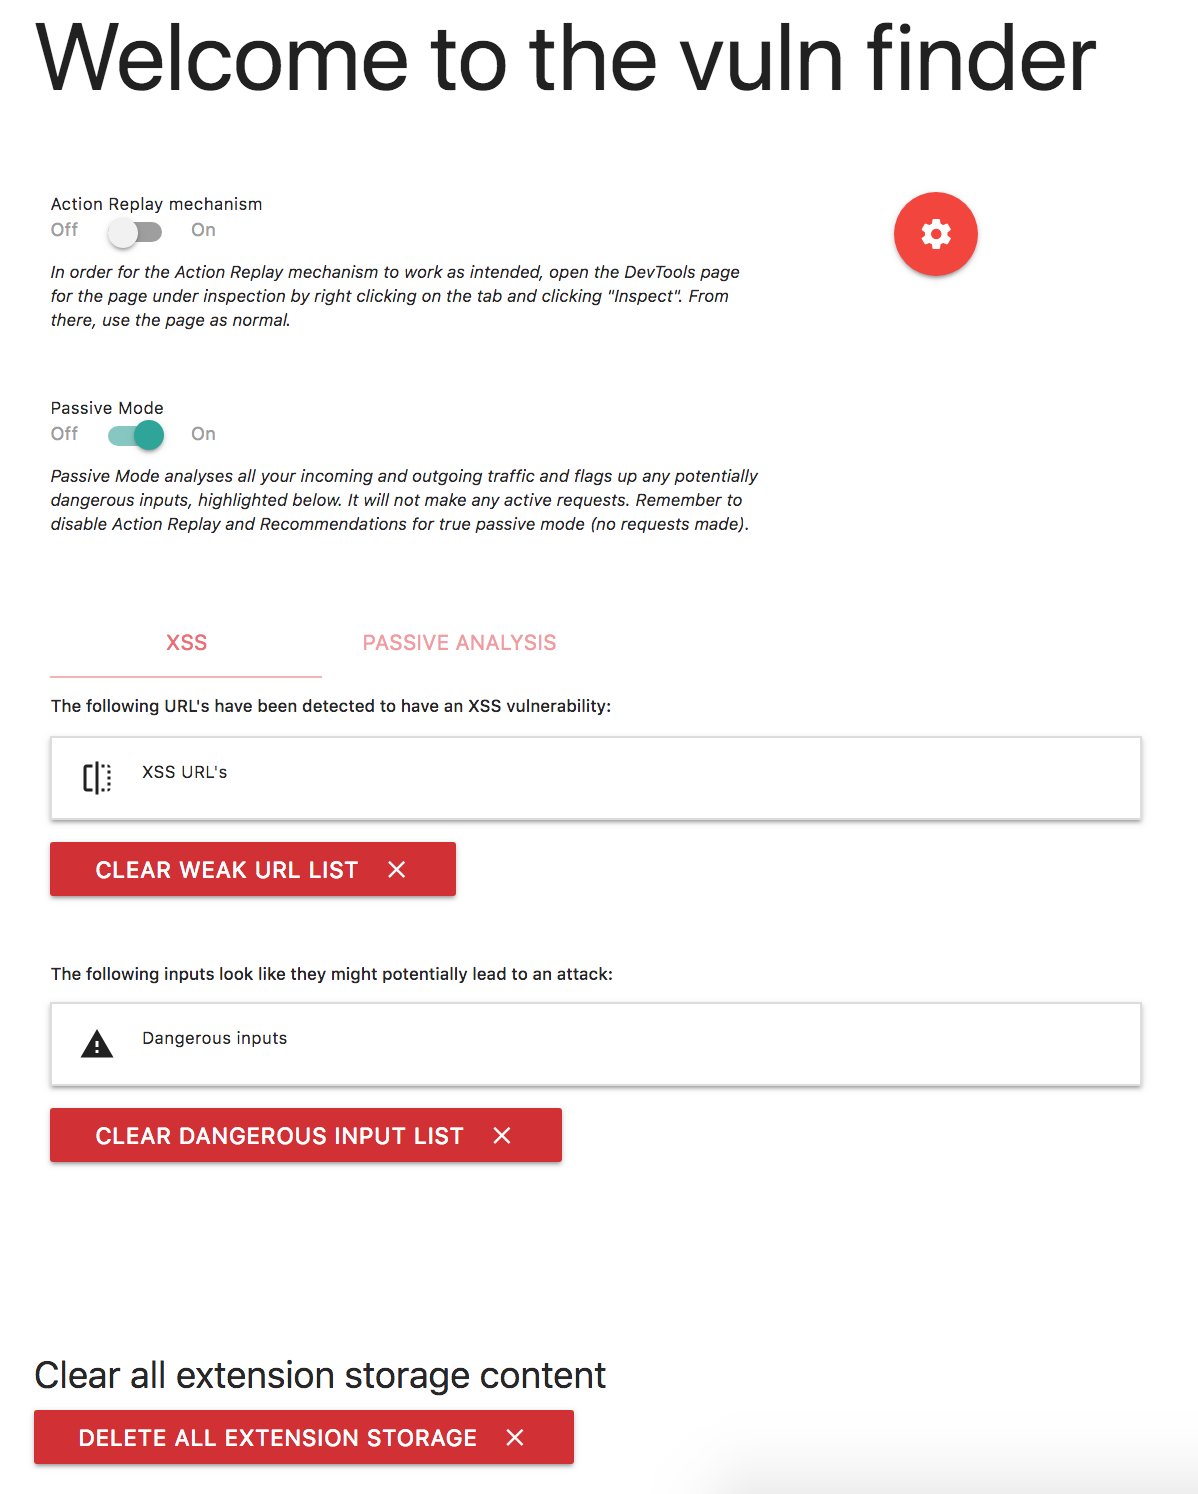
\includegraphics[width=0.8\textwidth]{images/popup_full.png}
	\caption{The main contents of the popup page when first clicked by a userw}
	\label{fig:test}
\end{figure}

This page offers an accessible means for tweaking and toggling all the options available in the extension, as well as viewing and analysing the outputs from the different modes of running the extension.  


\section{Background Page}

The background page I am using in the extension is a persistent page, meaning it is constantly running. This is in contrast to event background pages, which are opened and closed as necessary depending on the occasion. I am using this page to listen for messages sent from other scripts to be able to set aesthetic updates, as well as establishing a connection with the \texttt{devtools} page to subscribe to and forward custom request messages to content scripts.

\section{Request Logger}

This page is designed to capture information from attacks that have successfully hijacked Javascript execution and diverted a user to this page. In order to be accessible from any other window, it must be declared as a \texttt{web\_accessible\_resource}. It captures the page it was referred from and reports it as a page where a vulnerability exists.

\section{Devtools} \label{devtools}

The devtools page has access to a specific set of API's designed to extend the experience for web developers using the browser. This includes access to the currently inspected window, the developer panels, and network request information \cite{chromeExtensionDevTools}. \\

\begin{figure}[h]
	\centering
	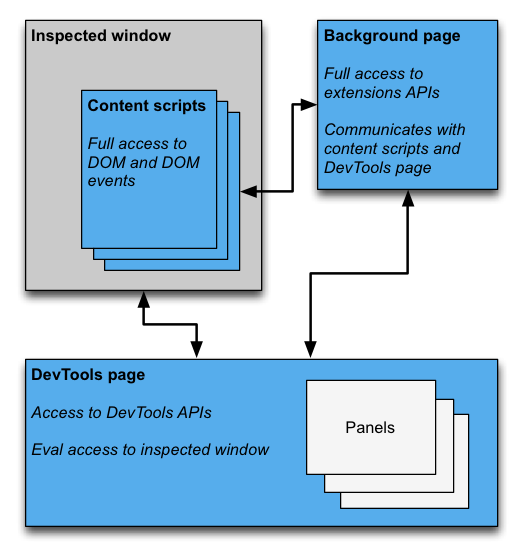
\includegraphics[width=0.55\textwidth]{images/devtools-extension.png}
	\caption{An extension making use of the DevTools API's further extends the capabilities of a standard Chrome Extension. Diagram from \cite{chromeExtensionDevTools}}
	\label{fig:test}
\end{figure}

More specifically, I am interested in the \texttt{devtools.network} API - this provides access to every request once it has finished. This contains a wealth of information which is otherwise difficult to obtain without using the devtools API. One of the APIs I am also using in the extension is the \texttt{chrome.webRequest}. This gives me access to several different events at different points of the lifetime of the request. It allows me to access some headers as well as change a limited set of these. It however does not provide sufficient information for the purposes of the extension - \texttt{devtools.network} gives access to the response content of any given request, which is vital in analysing outputs from a request to create attack correlations. Accessing the \texttt{devtools} APIs requires the Developer tools to be open for the page in question, which is only a small inconvenience when using the extension.

\section{Message Design}

To better understand the structure of the extension and how each feature ahead is to be implemented, it's good to create a high level overview of messaging between each component.  \\

\begin{figure}[h]
	\centering
	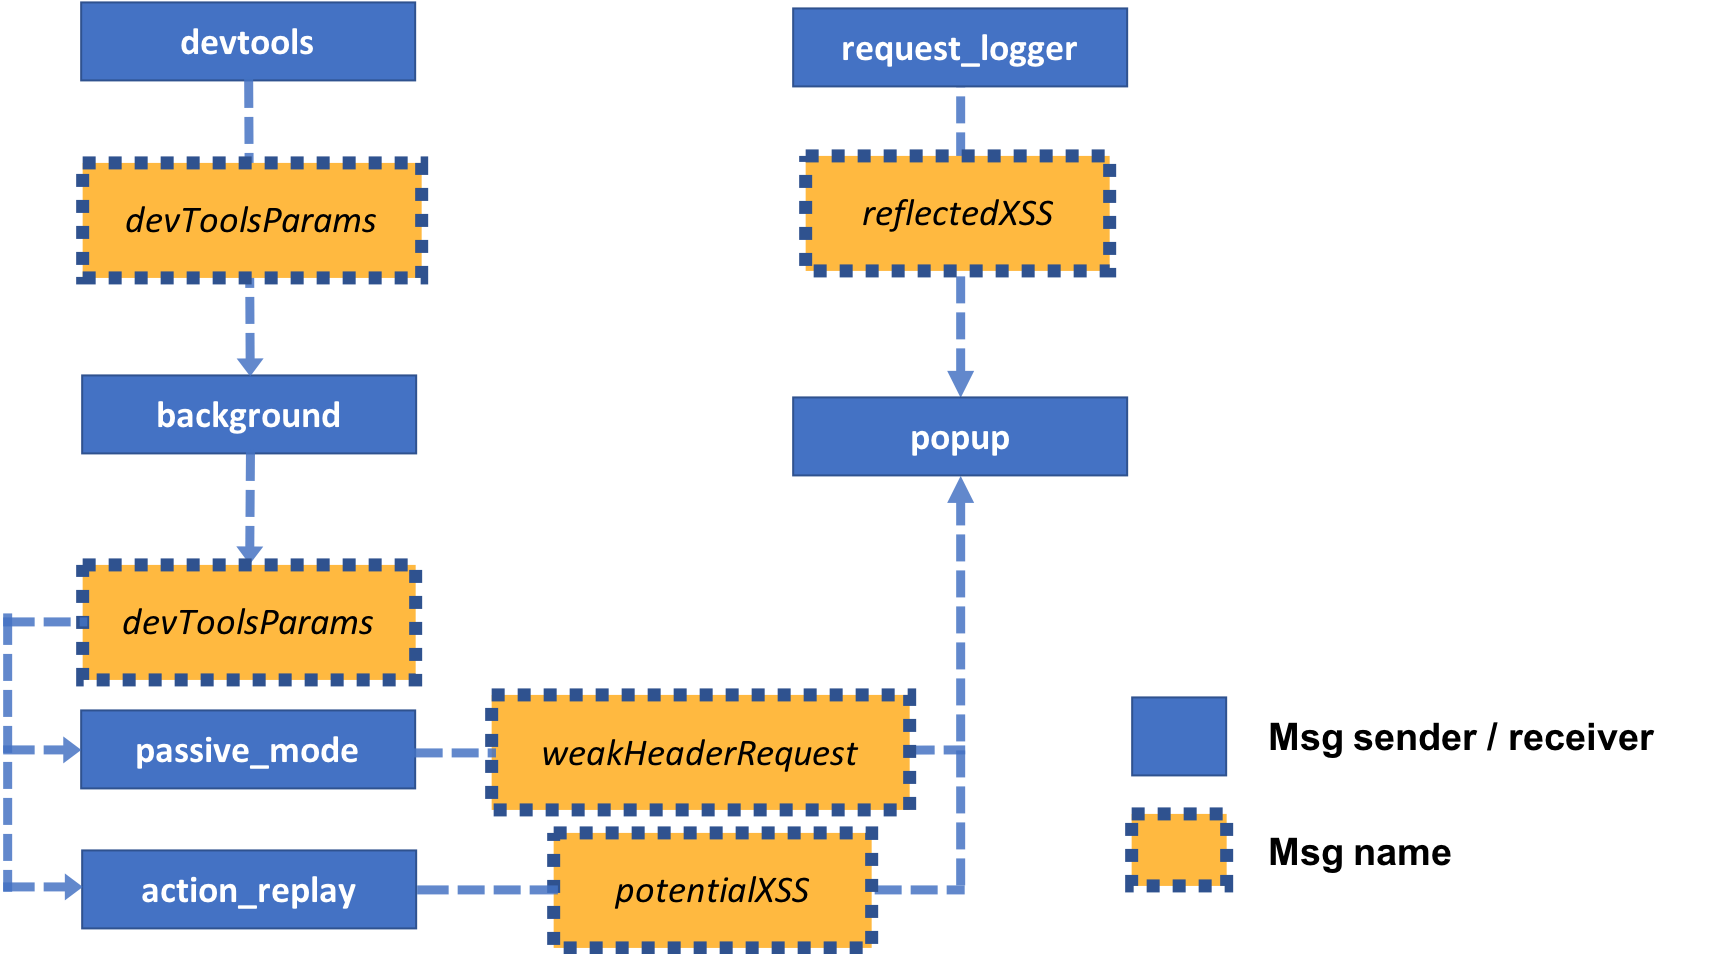
\includegraphics[width=0.95\textwidth]{images/message_passing.png}
	\caption{This diagram illustrates the passing of messages within the different components in the extension}
	\label{fig:test}
\end{figure}

In order to analyse the requests being made in different context scripts, the \texttt{devtools} script gathers every request made in the page which has the Developer Tools inspection windows open. Since this page cannot directly pass messages to the content scripts \cite{chromeExtensionDevTools}, it uses the background page as a mediator. It establishes a connection to the background page and passes to it every request it picks up. The background page then forwards these messages to the different content scripts that analyse the requests - \texttt{action\_replay} and \texttt{passive\_mode}. \\

Whenever a request causes the \texttt{request\_logger} page to be loaded, the page captures the information from the page it has just been referred to from, and forwards this information in a message to the \texttt{popup} page to update the list of vulnerable URLs. To toggle the enabling or disabling of the Action Replay algorithm, the popup page sends a message to the \texttt{action\_replay} script each time the corresponding switch is clicked. When the Action Replay is mid analysis, it will produce a warning list of inputs it has considered to be potentially dangerous, and passes a message to the \texttt{popup} page when it has detected this. Similarly, in the \texttt{passive\_mode} script, a message is passed to the \texttt{popup} alerting to any suspicious request behaviour. The \texttt{background} script also listens to several of these messages, and consequently updates the UI badge aesthetics, alerting the user to fresh information to analyse in the extension.


\section{Recommendations}

One of the large features intended for implementation in this project was the use of suggestions whilst browsing a page to attempt vulnerability exploits. This provides a low-effort means for a penetration tester to quickly test different types of attacks on a webpage. \\



I have implemented this by overriding every form on a page with an input of my own. 

\section{Action Replay}

The Action 


\section{Passive Mode}

Mention about 2 different ways of doing it - passive mode with normal cross checks by default - sliding window with eviction of requests.
Instead I keep window size and cross check only when enabled.

